\documentclass{article}
\usepackage{bera}% optional: just to have a nice mono-spaced font
\usepackage{listings}
\usepackage{xcolor}
\usepackage{amsmath}
\usepackage{graphicx}
\usepackage[colorlinks=true, allcolors=blue]{hyperref}
\usepackage[french]{babel}
\usepackage[a4paper, total={19cm,27.5cm}]{geometry}

\renewcommand{\thesection}{\Roman{section}}
\renewcommand{\thesubsection}{\thesection.\Roman{subsection}}

\definecolor{eclipseStrings}{RGB}{42,0.0,255}
\definecolor{eclipseKeywords}{RGB}{127,0,85}
\colorlet{numb}{magenta!60!black}

\lstdefinelanguage{json}{
    basicstyle=\normalfont\ttfamily,
    commentstyle=\color{eclipseStrings}, % style of comment
    stringstyle=\color{eclipseKeywords}, % style of strings
    numbers=left,
    numberstyle=\scriptsize,
    stepnumber=1,
    numbersep=8pt,
    showstringspaces=false,
    breaklines=true,
    frame=lines,
    backgroundcolor=\color{white}, %only if you like
    string=[s]{"}{"},
    comment=[l]{:\ "},
    morecomment=[l]{:"},
    literate=
        *{0}{{{\color{numb}0}}}{1}
         {1}{{{\color{numb}1}}}{1}
         {2}{{{\color{numb}2}}}{1}
         {3}{{{\color{numb}3}}}{1}
         {4}{{{\color{numb}4}}}{1}
         {5}{{{\color{numb}5}}}{1}
         {6}{{{\color{numb}6}}}{1}
         {7}{{{\color{numb}7}}}{1}
         {8}{{{\color{numb}8}}}{1}
         {9}{{{\color{numb}9}}}{1}
}

\title{Compte-rendu projet informatique : Simulation à N corps et système solaire}
\author{COUËRON Lola \\ JOLY Marine \\ \\ L3 Physique, Université Grenoble Alpes}

\begin{document}
\maketitle

{
\hypersetup{hidelinks}

\renewcommand{\contentsname}{Sommaire}
\tableofcontents
}

\section{Introduction}
    \subsection{Contexte}
    La simulation informatique est un outil de plus en plus utilisé dans l'étude des phénomènes physiques puisqu'elle permet de comparer de façon efficace des modèles théoriques aux résultats expérimentaux. Celle-ci permet également de simuler des expériences qui ne sont pas réalisables en pratique. Dans ce cadre, nous avons développé une simulation à N corps en Python. En partant de la modélisation de l'interaction Terre-Soleil avec les équations de Newton puis d'une simulation du système solaire à l'aide de l'algorithme de Runge-Kutta d'ordre 4, nous avons créé un logiciel qui permet de personnaliser des simulations avec autant de corps que souhaité.

    \subsection{Structure générale du code}
    Ce projet étant collaboratif, nous avons travaillé sur \href{https://github.com/MJ240103/solarSystem}{GitHub} (https://github.com/MJ240103/solarSystem) afin d'optimiser la répartition des tâches. Ce projet est divisé en 4 fichiers : \\

    \begin{enumerate}
        \item le fichier contenant l'application réalisée avec Tkinter (UIsolarSystem.py)
        \item le fichier contenant la simulation réalisée avec PyGame (mainEngine.py)
        \item le fichier contenant les équations et les paramètres physiques nécessaires à la simulation (bodies.py)
        \item les fichier permettant de stocker les paramètres de simulations déjà existantes (fichiers json d'extension .mj et Simulation1.py)
    \end{enumerate}

    \\

    \begin{figure}[h]
        \centering
        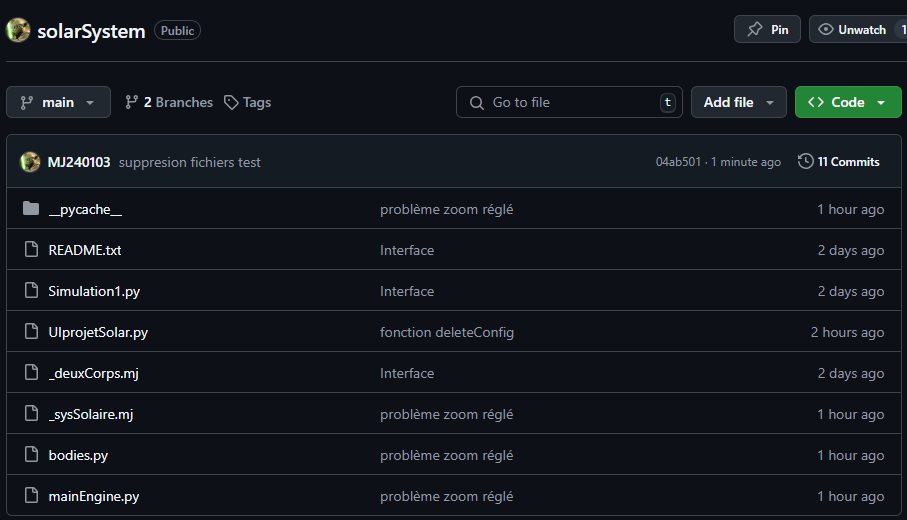
\includegraphics[width=0.5\linewidth]{imgGitHub.png}
        \caption{\label{fig:Git}Fichiers de la branche main du repository solarSystem.}
    \end{figure}

    \\

    Le fichier mainEngine.py utilise les équations et paramètres physiques du fichier bodies.py afin de simuler les intéractions attractives entre un certain nombre de corps et avec certains paramètres par le biais de PyGame. Ce nombre de corps et ces paramètres seront définis par l'utilisateur grâce à l'interface contenue dans le fichier IUsolarSystem. Celle-ci utilise Tkinter pour lancer la simulation PyGame. Les simulations peuvent être stockées dans des fichiers python (ex : Simulation1.py) ou dans des fichiers json (ex : sysSolaire.mj).

\section{Partie physique}

    Le fichier bodies.py contient tous les paramètres physiques et fonctions nécessaires à la simulation.
    
    \subsection{Implémentation naïve}

        Au commencement, nous avons opté pour une implémentation naïve des équations du mouvement. Nous considérions un corps central autour duquel gravite un autre corps. Le mouvement de ce corps était régi par la force de gravitation $\vec{F} = \frac{-G m_A m_B}{r^2} \vec{U_r}$.

        \paragraph{}

        Les coordonnées cartésiennes ont été utilisées afin de simplifier l'implémentation des équations du mouvement en Python. \\
        La position d'une particule en coordonnées cartésiennes est donnée par :
        \begin{equation}
            \vec{r}(t) = x(t) \vec{i} + y(t) \vec{j} + z(t) \vec{k}
        \end{equation}. \\
        La vitesse est la dérivée de la position par rapport au temps :
        \begin{equation}
            \vec{v}(t) = \frac{d\vec{r}(t)}{dt} = \frac{dx(t)}{dt} \vec{i} + \frac{dy(t)}{dt} \vec{j} + \frac{dz(t)}{dt} \vec{k}
        \end{equation}. \\    
        L'accélération est la dérivée de la vitesse par rapport au temps :
        \begin{equation}
            \vec{a}(t) = \frac{d\vec{v}(t)}{dt} = \frac{d^2x(t)}{dt^2} \vec{i} + \frac{d^2y(t)}{dt^2} \vec{j} + \frac{d^2z(t)}{dt^2} \vec{k}
        \end{equation}.

        
        Nous avons appliqué le Principe Fondamental de la Dynamique (PFD) $\vec{F} = m \vec{a}$ au corps en orbite, puis projetté celui-ci dans le repère cartésien afin d'obtenir l'équation du mouvement en coordonnées cartésiennes.

        \paragraph{}
        Enfin, nous avons implémenté ces équations en Python. L'appel à la fonction applyGravity effectue les calculs de position, de vitesse et d'accélération du corps en orbite. Quant à la fonction setPosition, celle-ci est chargée de mettre à jour la position du corps en orbite en fonction de sa vitesse et de l'intervalle de temps indiquant la durée d'une révolution autour de l'astre central.

        \begin{center}
            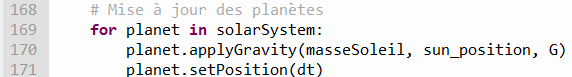
\includegraphics[scale=0.5]{naifMain.png} \\
            \emph{Exécution des fonctions setPosition et applyGravity pour créer les coordonnées nécessaires pour la simulation dans mainEngine.py}
        \end{center}

        \begin{center}
            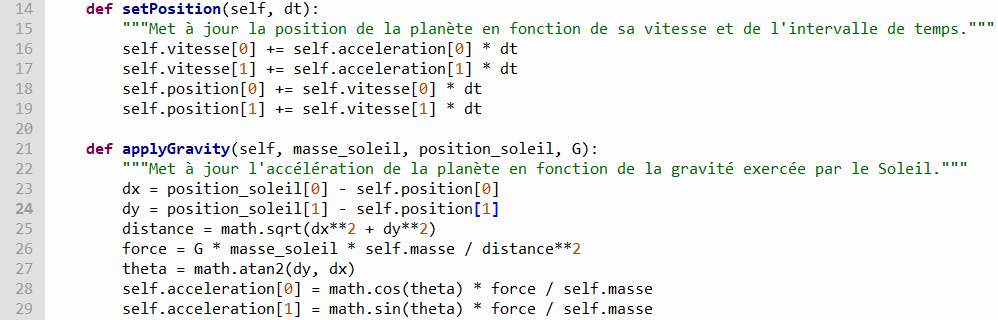
\includegraphics[scale=0.5]{naif.png} \\
            \emph{Fonctions setPosition et applyGravity du module bodies.py}
        \end{center}

    \subsection{Implémentation avec Runge-Kutta d'ordre 4}

        Voyant les limites de l'implémentation naïve, nous nous sommes intéréssées aux différents algorithmes qui permettent de modéliser un mouvement numériquement. Au cours de nos recherches, deux algorithmes ont particulièrement attiré notre attention : Euler et Runge-Kutta d'ordre 4 (RK4).

        \paragraph{}

         La méthode d'Euler est une procédure numérique pour résoudre par approximation des équations différentielles du premier ordre avec une condition initiale. La méthode d'Euler a l'avantage d'être simple mais l'erreur induite peut être assez élevée si le pas est choisi trop grand, ce qui implique donc de devoir faire énormément de calculs pour atteindre une précision acceptable.

          \paragraph{}

            Par conséquent, nous nous sommes tout naturellement tournées vers la méthode RK4. En effet, cette méthode d'analyse numérique d'approximation de solutions d'équations différentielles repose sur le principe de l'itération, c'est-à-dire qu'une première estimation de la solution est utilisée pour calculer une seconde estimation, plus précise, et ainsi de suite. La méthode RK4 est une méthode d'ordre 4, ce qui signifie que l'erreur commise à chaque étape est de l'ordre de h5, alors que l'erreur totale accumulée est de l'ordre de h4. Ainsi, elle est bien plus précise que la méthode d'Euler.

            \paragraph{}

            On considère le problème suivant : $y' = f(t,y)$ avec $y(t_0) = y_0$.

            \paragraph{}

            La méthode RK4 est donnée par l'équation : $y_{n+1} = y_n + \frac{h}{6} (k_1 + 2k_2 + 2k_3 + k_4)$
            
            où
            
            \begin{itemize}
                \item $k_1 = f(t_n, y_n)$
                \item $k_2 = f(t_n + \frac{h}{2}, y_n + \frac{h}{2} k_1)$
                \item $k_3 = f(t_n + \frac{h}{2}, y_n + \frac{h}{2} k_2)$
                \item $k_4 = f(t_n + h, y_n + hk_3)$
            \end{itemize}

            \paragraph{}

            Le fonctionnement se base sur l'idée que la valeur suivante ($y_{n+1}$) est approchée par la somme de la valeur courante ($y_n$) et du produit de la taille de l'intervalle (h) par la pente estimée. Cette pente est obtenue en effectuant une moyenne pondérée de pentes : \\

            \begin{itemize}
                \item $k_1$ correspond à la pente au début de l'intervalle.
                \begin{center}
                    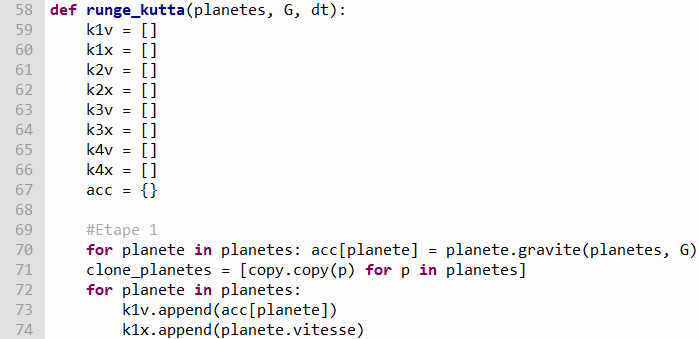
\includegraphics[scale=0.5]{RK4partie1.png} \\
                    \emph{Etape 1 de la méthode RK4.}
                \end{center}
                \item $k_2$ correspond à la pente au milieu de l'intervalle. Elle s'obtient en utilisant $k_1$ pour calculer la valeur de $y$ au point $t_n + \frac{h}{2}$ par le biais de la méthode d'Euler.
                \begin{center}
                    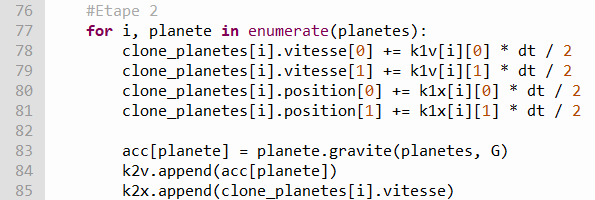
\includegraphics[scale=0.5]{RK4partie2.png} \\
                    \emph{Etape 2 de la méthode RK4.}
                \end{center}
                \item $k_3$ est la pente au milieu de l'intervalle, mais obtenue en utilisant $k_2$ pour $y$.
                \begin{center}
                    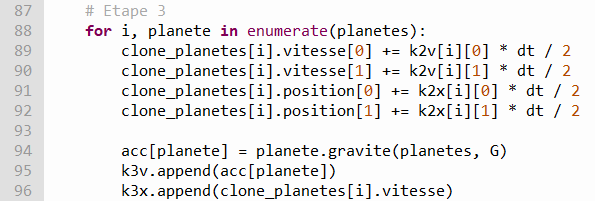
\includegraphics[scale=0.5]{RK4partie3.png} \\
                    \emph{Etape 3 de la méthode RK4.}
                \end{center}
                \item $k_4$ correspond à la pente de la fin de l'intervalle, obtenue avec la valeur de $y$ calculée en utlisant $k_3$.
                \begin{center}
                    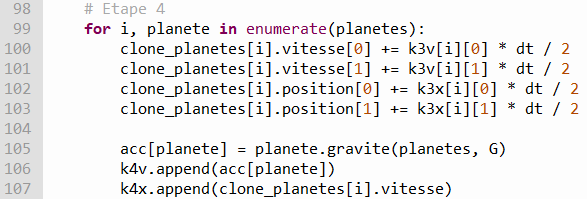
\includegraphics[scale=0.5]{RK4partie4.png} \\
                    \emph{Etape 4 de la méthode RK4.}
                \end{center}
            \end{itemize}

            \paragraph{}

            Lorsque la moyenne pondérée des 4 pentes est effectuée, un poids plus important est donné aux pentes du milieu.

             \begin{center}
                    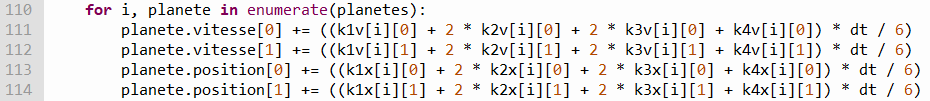
\includegraphics[scale=0.5]{RK4partiefin.png} \\
                    \emph{Intération de la méthode RK4.}
                \end{center}

            La méthode RK4 est une méthode d'ordre 4. Ainsi, l'erreur commise à chaque étape est de l'ordre de $h^5$, tandis que l'erreur totale accumulée est de l'ordre de $h^4$. Par conséquent, l'erreur est suffisament faible pour avoir des simulations précises et proches de la réalité.

\section{Partie simulation}

\section{Partie interface}
    \subsection{Paramétrage des simulations}

    \paragraph{Body.}
    Nous appelons \emph{Body} un objet regroupant les caractéristique suivante: 

    \begin{itemize}
        \item Nom (string) : Nom de l'objet
        \item Masse (float) : Masse de l'objet
        \item Rayon (float) : Rayon de l'objet
        \item Position (float tuple) : Position (cartésienne) de l'objet
        \item Vitesse (float tuple) : Vitesse (cartésienne) de l'objet
        \item Acceleration (float tuple) : Accélération (cartésienne) de l'objet
        \item couleur ( int 3-uplet) : Couleur
    \end{itemize}

    Un \emph{Body} peut par exemple représenter la terre, le soleil, un satellite artificiel...

    \paragraph{Simulation.}
    Nous appelons \emph{Simulation} un objet regroupant les caractéristiques suivantes:

    \begin{itemize}
        \item Nom\_Simu (string) : Nom de la simulation
        \item FPS (int) : Frame Per Second (nombre d'image par seconde) de la simulation
        \item G (float) : Constante gravitationnelle
        \item dt (float) : Intervalle de temps utilisé par RK4
        \item SPACE\_X (float) : Taille horizontale de l'espace simulé
        \item SPACE\_Y (float) : Taille vecticale de l'espace simulé
        \item ECHELLE\_RAYON (float) : Echelle de rendu des rayons des \emph{body}
        \item UNIVERSE\_CENTER (float tuple) : Centre de l'univers (au centre de l'affichage en début de simulation)
        \item planetes (\emph{Body} list) : Liste des objets, tels que définit avec le constructeur \emph{body}
    \end{itemize} \\

    Pour enregistrer une simulation, nous utilisons le format \empj{JavaScript Object Notation} (JSON). 

    Python a l'avantage de directement prendre en charge ce format à l'aide du module Json. Ainsi, en important le fichier simulation et en signifiant à python qu'il s'agit de json, on peut accéder aux différents paramètres de la simulation.

    On accède par exemple au nom d'une simulation représentée par la variable sim de la manière suivante: nomSimu = sim["Nom\_Simu"]
    
    \begin{center}
        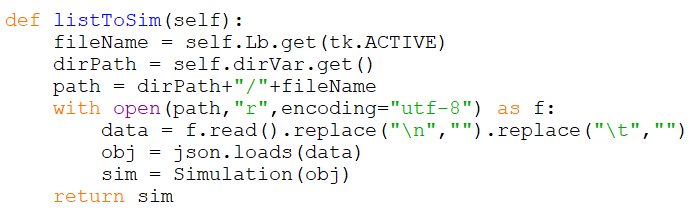
\includegraphics[scale=0.7]{toJson.png} \\   
        \emph{Importation d'un fichier via le module Json}
    \end{center}

    Nous transformons ensuite notre objet directement convertis depuis le Json en un objet Simulation à l'aide d'une classe. L'avantage de cette méthode est que la classe Simulation possède une méthode \emph{launch()} qui lance directement l'execution de la simulation dans le moteur.
    
    \begin{center}
        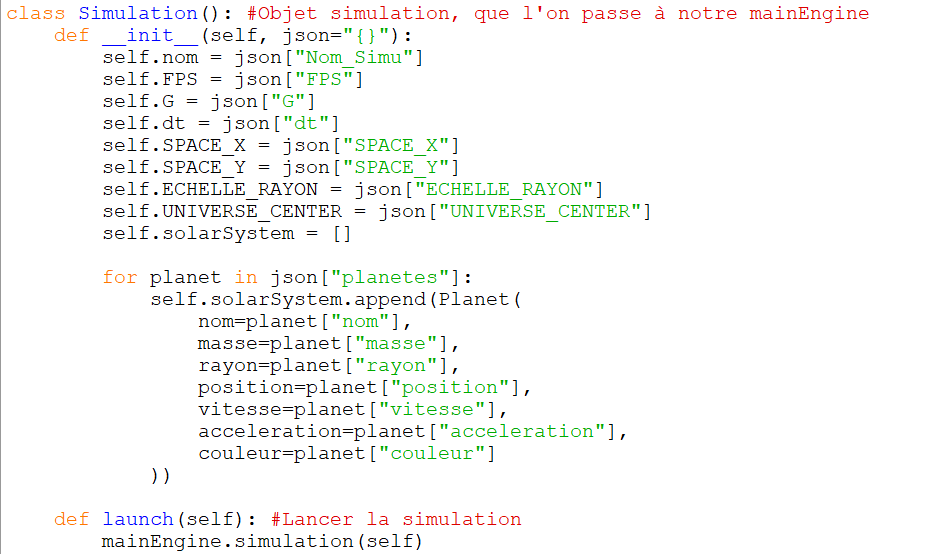
\includegraphics[scale=0.5]{simulationClasse.png} \\   
        \emph{Classe Simulation}
    \end{center}

    \subsection{Modification, Création}

    L'interface, réalisée à l'aide de Tkinter se présente comme suit:

    \begin{center}
        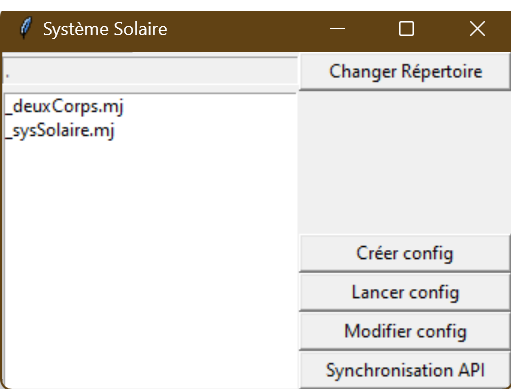
\includegraphics[scale=0.5]{mainInterface.png}\\    
        \emph{Interface - Fenetre principale}
    \end{center}

    Sur la fenêtre principale de l'interface, on a la possibilité de se placer dans un répertoire en cliquant sur "Changer Répertoire". Le répertoire par défaut est celui est du fichier interface.

    La \emph{ListBox} a gauche liste les fichiers de simulations compatibles (.mj) dans le répertoire courant. Ces fichiers contiennent un code JSON correspondants à l'objet \emph{Simulation} définit plus haut. 

    Lorsqu'on clique sur le nom d'un fichier, il devient le fichier actif. On peut ensuite cliquer sur:

    \begin{itemize}
        \item "Lancer config" : Execute la configuration dans l'engine
        \item "Modifier config" : Ouvre la fenetre secondaire avec les paramètres de la simulation active.
    \end{itemize}

    Indépendament du fichier actif, on peut cliquer sur:

    \begin{itemize}
        \item "Créér config" : Ouvre la fenetre secondaire avec les paramètres par défaut.
        \item "Synchronisation API" : Récupère les positions et vitesse actuelles des astres du système solaire , créé un fichier de simulation, et l'execute.
    \end{itemize}

    \begin{center}
        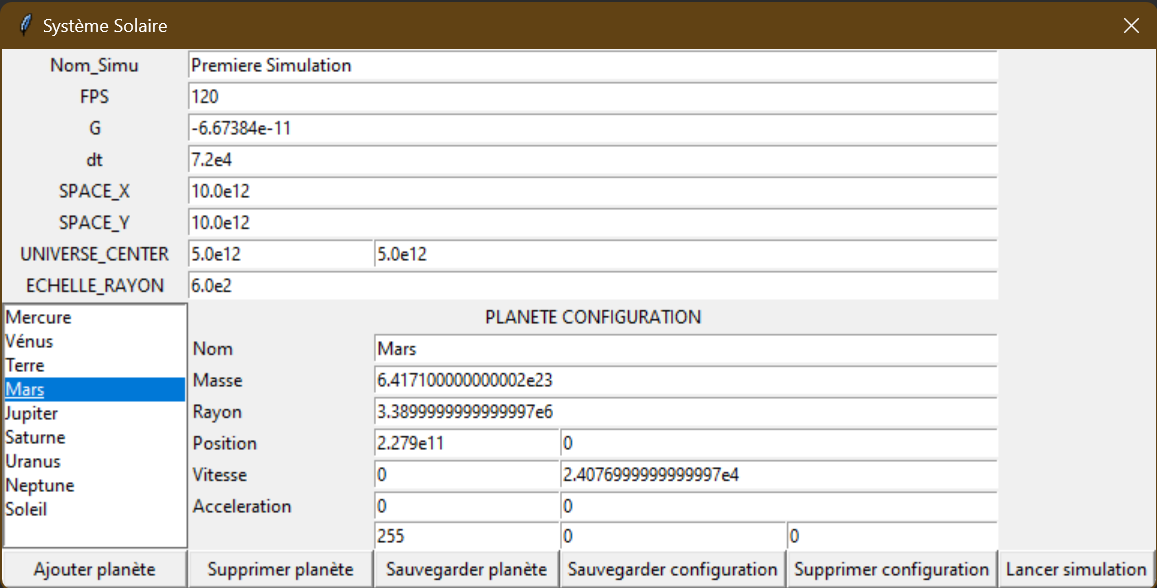
\includegraphics[scale=0.5]{interfaceFenetreSecondaire.png}\\    
        \emph{Interface - Fenetre secondaire}
    \end{center}

    Cette fenetre secondaire s'ouvre soit lorsqu'on souhaite modifier une simulation existante, soit à la création d'une nouvelle simulation. Dans les deux cas, elle se comporte de la même manière. 

    L'édition de constante se fait simplement en modifiant les champs associés. 

    L'édition des planètes se fait en cliquant sur le nom de la planète à modifier, en éditant les champs, puis en cliquant sur "Sauvegarder planète". 

    On peut également "Ajouter planète" ou "Supprimer planète".

    Une fois les modifications effectuées, on clique sur "Sauvegarder configuration", qui nous ouvre une fênetre de dialogue windows pour sauvegarder le fichier simulation. On pourra alors écraser l'ancien (cas de modification), ou le lancer. 

    On peut aussi tester notre simulation modifiée avant de la sauvegarder, en cliquant sur "Lancer Simulation".

\section{Exemples d'application}
    \subsection{Cas à deux corps}

    \subsection{Cas du système solaire}

\section{Conclusion et ouverture}


\end{document}